\documentclass[10pt]{article}
\usepackage{amsfonts, amssymb, amsmath, amsthm, mathtools, enumerate, latexsym, setspace}
\usepackage[T1]{fontenc}
\usepackage[a4paper, total={7in, 10.5in}]{geometry}
\pagestyle{empty}

\usepackage{float}
\usepackage{pgfplots}
\pgfplotsset{compat=1.18}

\newcommand{\R}{\mathbb{R}}
\newcommand{\N}{\mathbb{N}}
\newcommand{\Z}{\mathbb{Z}}
\newcommand{\Q}{\mathbb{Q}}
\newcommand{\Prime}{\mathbb{P}}
\newcommand{\Pows}{\mathcal{P}}
\newcommand{\cont}{\mathfrak{c}}

\newcommand{\Dis}{\displaystyle}
\newcommand{\half}{\frac{1}{2}}
\newcommand{\Forall}{{\Large\mbox{$\forall$}}}
\newcommand{\Exists}{{\Large\mbox{$\exists$}}}

\title{PMat - wspólna praca domowa seria III}
\author{Gracjan Barski, album: 448189}
\date{January 22, 2024}

\begin{document}
\maketitle
% \onehalfspacing
\begin{center}
    W poniższych rozumowaniach moc zbioru oznaczam modułami, to znaczy moc zbioru $A$ to $|A|$, oraz zaliczam $0$ do liczb naturalnych.
\end{center}
\textbf{Zadanie 309:}
\begin{enumerate}[a)]
    \item Pokazać, że $r$ jest relacją równoważności. \\[10pt]
    Weźmy funkcję $h \colon \Z [x] \to \Z [x]$. Ta funkcja otrzyma wielomian na wejściu i wszystkie jego współczynniki zredukuje $\mod 2$. Traktując wielomian jako wektor w przestrzeni liniowej nad $\Z$ to można zapisać:
    $$h\left(\begin{bmatrix}
        x_1 \\
        x_2 \\
        \vdots \\
        x_n
    \end{bmatrix}\right) = \begin{bmatrix}
        x_1 \mod 2 \\
        x_2 \mod 2\\
        \vdots \\
        x_n \mod 2
    \end{bmatrix}$$
    Łatwo zaważyć że $r = \ker h$. Prosty dowód poprzez wzajemną inkluzję: \\[5pt]
    $(\subseteq)$ weźmy taką parę $\langle f, g \rangle \in r$. Wiemy że ich odpowiadające współczynniki mają taką samą parzystość (bo tylko różnica dwóch liczb o tej samej parzystości daje wynik parzysty). Korzystając z faktu że dwie liczby $a,b \in \Z$ spełniają równość $a \equiv b \mod 2$ wtedy i tylko wtedy gdy ich parzystość jest taka sama otrzymujemy $h(f) = h(g)$, czyli $\langle f, g \rangle \in \ker h$. \\[5pt]
    $(\supseteq)$ weźmy taką parę $\langle f, g \rangle \in \ker h$. Korzystając z tych samych dwóch faktów co wyżej wnioskujemy że ich odpowiadające współczynniki mają taką samą parzystość. Czyli ich różnica będzie miała tylko współczynniki parzyste, więc $\langle f, g \rangle \in r$. \\[5pt]
    Z wzajemnej inkluzji wnioskujemy równość zbiorów. \\[5pt]
    Z wykładu wiadomo że relacja jest relacją równoważności wtedy i tylko wtedy gdy istnieje funkcja, której ta relacja jest jądrem, więc wnioskujemy że $r$ jest relacją równoważności. \qed
    \vspace{10pt}
    
    \item Wskazać trzy różne klasy abstrakcji.
    \begin{enumerate} [1)]
        \item $[0]_r$ zbiór wszystkich wielomianów o współczynnikach parzystych

        \item $[1]_r$ zbiór wszystkich wielomianów które przy $x^0$ mają współczynnik nieparzysty, a pozostałe współczynniki parzyste

        \item $[x + 1]_r$ zbiór wszystkich wielomianów które przy $x^0$ i $x^1$ mają współczynniki nieparzyste, a pozostałe współczynniki parzyste
    \end{enumerate}

    \item Wyznaczyć moc zbioru $\Z [x]/_r$. \\[10pt]
    Rozważmy funkcję $f \colon \Pows_{\text{fin}} (\N) \to \Z[x]/_r$ określoną wzorem 
    $$f(A) = \left[\sum_{n=0}^{\max A} \chi_A (n) \cdot x^n\right]_r$$ 
    Gdzie $\Pows_{\text{fin}}(\N)$ to zbiór wszystkich skończonych podzbiorów $\N$, a $\chi_A$ to indykator zbioru $A$. Biorę tylko skończone podzbiory $\N$, ponieważ gdybym wziął wszystkie to argument funkcji mógłby nie mieć elementu największego, a jeżeli suma we wzorze iterowałaby do nieskończoności to otrzymany obiekt nie byłby wielomianem, więc byłby poza dziedziną (wielomiany muszą mieć skończony stopień). \newpage
    Pokażę, że $f$ jest iniekcją. \\[5pt]
    Weźmy dwa dowolne $A_1, A_2 \in \Pows(\N)$ takie że $A_1 \neq A_2$, to oznacza że w którymś jest element, którego nie ma w drugim. Bez straty ogólności załóżmy $\Exists_{a_1 \in A_1} \; a_1 \notin A_2$. Weźmy to $a_1$. Rozważmy wartość $f(A_1)$:
    $$f(A_1) = \left[\sum_{n=0}^{\max A_1} \chi_{A_1} (n) \cdot x^n\right]_r = \left[ \chi_{A_1}(0) \cdot x^0 + \chi_{A_1}(1) \cdot x^1 + \ldots + \chi_{A_1}(a_1) \cdot x^a_1 + \ldots + \chi_{A_1}(\max A_1) \cdot x^{\max A_1}\right]$$
    Jako że $\chi_{A_1}(a_1) = 1$, to wielomiany w $f(A_1)$ mają współczynniki nieparzyste przy $x^{a_1}$. W przeciwieństwie do tego, wszystkie wielomiany w $f(A_2)$ mają współczynniki parzyste (bo $\chi_{A_2}(a_1) = 0$), więc wnioskujemy, że:
    $$\left\langle \sum_{n=0}^{\max A_1} \chi_{A_1} (n) \cdot x^n, \sum_{n=0}^{\max A_2} \chi_{A_2} (n) \cdot x^n \right\rangle \notin r$$
    A jeśli nie są ze sobą w relacji $r$ to ich klasy abstrakcji są różne (ponieważ $r$ jest relacją równoważności), więc istotnie $f$ jest iniekcją. \\[10pt]
    Teraz pokażę, że $f$ jest surjekcją: \\[5pt]
    Weźmy klasę abstrakcji $[p]_r$, dla dowolnego $p \in \Z[x]$. Weźmy wielomian $p' \in \Z[x]$, który spełnia $p' = h(p)$ (gdzie funkcja $h$ to funkcja zdefiniowana w podpunkcie a)). Czyli $p'$ to po prostu wielomian ze zredukowanymi $\mod 2$ współczynnikami wielomianu $p$. Jak wykazano w podpunkcie wcześniejszym, $p$ i $p'$ są ze sobą w relacji $r$, więc $[p]_r = [p']_r$. Więc teraz będziemy rozpatrywać klasę abstrakcji $[p']_r$. Biorę $p'$ i sprawdzam przy jakich potęgach $x$ ma on współczynniki równe 1, a następnie te potęgi umieszczam w zbiorze $A$. Formalnie:
    $$A = \{ n \in \N \mid \text{współczynnik $p'$ przy $x^n$ jest równy 1} \}$$
    Dla ścisłości warto zaznaczyć, że taki zbiór jest skończony, ponieważ wielomiany mają skończony stopień, więc istotnie $A \in \Pows_{\text{fin}}(\N)$. Z własności $f$ mamy: $f(A) = [p']_r = [p]_r$ więc istotnie $f$ jest surjekcją. \\[10pt]
    Więc $f$ jest bijekcją, a to oznacza, że $\Pows_{\text{fin}} (\N) \sim \Z[x]_r$. Z ćwiczeń wiadomo że $|\Pows_{\text{fin}} (\N)| = \aleph_0$, więc wnioskujemy: $|\Z[x]/_r| = \aleph_0$. \qed
    \vspace{10pt}
    
    \item Wskazać wszystkie liczby kardynalne, które są mocami klas abstrakcji tej relacji. \\[10pt]
    Weźmy klasę abstrakcji $[p]_r$ dla dowolnego $p \in \Z[x]$.\\[5pt] Rozważmy funkcję identycznościową $f_p \colon [p]_r \to \Z[x]$ zadaną wzorem $f(p) = p$. Z oczywistych względów ta funkcja jest iniekcją. Więc wnioskujemy, że $|[p]_r| \leq |\Z[x]|$. Wiemy że $|\Z[x]| = \aleph_0$ (fakt z wykładu), więc mamy $|[p]_r| \leq \aleph_0$. Teraz potrzebujemy dolnego ograniczenia, jednak jest ono trywialne.\\[5pt]
    Pokażę, że dla dowolnej takiej klasy $[p]_r$ mamy w niej nieskończenie wiele elementów. Skorzystam z faktu, że wielomian jest wyznaczony unikalnie przez jego współczynniki. Weźmy ten wielomian $p$ oraz jego pewien współczynnik $a_i$ przy $x^i$. Teraz weźmy wielomian $p'$, który ma wszystkie współczynniki te same co $p$, oprócz tego $a_i$. Chcielibyśmy żeby $p' \in [p]_r$, więc jeśli za współczynnik przy $x^i$ wezmę $a_i + 2k$ dla dowolnego $k \in \Z$, to faktycznie $p' \in [p]_r$ (ponieważ $a_i + 2k - a_i \equiv 0 \mod 2$ dla każdego $k \in \Z$). Więc mam do wyboru $\aleph_0$ współczynników, więc istotnie klasa abstrakcji $[p]_r$ jest nieskończona. A z tego wnioskuję, że $\aleph_0 \leq |[p]_r|$ (ponieważ $\aleph_0$ to najmniejsza możliwa nieskończoność).\\[5pt]
    Z twierdzenia Cantora-Bernsteinta otrzymuję $|[p]_r| = \aleph_0$ dla każdego $p \in \Z[x]$. \qed
    
\end{enumerate}

\vspace{20pt}

\textbf{Zadanie 336:}
\newcommand{\Rel}{\mathcal{R}}
\begin{enumerate}[a)]
    \item Znaleźć $\displaystyle \bigcup_{r \in \Rel} \; g(r)$ i $\displaystyle \bigcap_{r \in \Rel} \; g(r)$ \\[10pt]
    Najpierw pokażę, że $\bigcup_{r \in \Rel} \; g(r) = \Pows (\N)$. Prosty dowód poprzez wzajemną inkluzję: \\[5pt]
    $(\subseteq)$ Weźmy dowolne $A \in \bigcup_{r \in \Rel} \; g(r)$. Z definicji mamy $\Exists_{r \in \Rel} \; A \in g(r)$, a to oznacza że w szczególności $A \in \Pows(\N)$, ponieważ $g(r)$ jest typu $\Pows(\Pows(\N))$. \\[5pt]
    $(\supseteq)$ Weźmy dowolne $A \in \Pows(\N)$. Weźmy taką relację równoważności $r \in \Rel$ której jedną z klas abstrakcji jest zbiór $A$, a drugą $\N - A$. Wtedy $g(r) = \{A, \N - A\}$, więc $A \in r$, a z tego $A \in \bigcup_{r \in \Rel} \; g(r)$. \\[5pt]
    Z wzajemnej inkluzji wnioskujemy równość zbiorów. \\[10pt]
    Teraz pokażę, że $\bigcap_{r \in \Rel} \; g(r) = \varnothing$. \\[5pt]
    Załóżmy nie wprost, że $\bigcap_{r \in \Rel} \; g(r)$ jest niepuste. To oznacza, że istnieje $A \in \Pows(\N)$ takie że $\Forall_{r \in \Rel} \; A \in g(r)$, czyli innymi słowy $A$ jest klasą abstrakcji w każdej relacji $r \in \Rel$. Rozważmy dwa przypadki:
    \begin{enumerate}[1)]
        \item $A$ jest singletonem: Wtedy $A$ nie należy do $g(\N^2)$, ponieważ relacja $\N^2$ posiada tylko jedną klasę abstrakcji, która nie jest singletonem (a mianowicie cały zbiór $\N$).

        \item $A$ nie jest singletonem: Wtedy $A$ nie należy do $g(\mathbf{1}_\N)$, ponieważ relacja $\mathbf{1}_\N$ posiada tylko klasy abstrakcji które są singletonami.
    \end{enumerate}
    Mamy sprzeczność w obu przypadkach, więc takie $A$ nie istnieje, a to oznacza że $\bigcap_{r \in \Rel} \; g(r) = \varnothing$. \qed

    \item Czy $g$ jest iniekcją? Czy jest surjekcją? \\[10pt]
    Wykażę iniektywność $g$: \\[5pt]
    Wiadomo, że każda relacja równoważności na danym zbiorze jest definiowana \textbf{unikalnie} przez podział na tym zbiorze (fakt z wykładu), więc jeśli wezmę dwie relacje równoważności $r_1, r_2 \in \Rel$ takie że $r_1 \neq r_2$, to są one zdefiniowane przez dwa różne podziały $\N$. Warto zauważyć, że funkcja $g(r)$, mapuje $r$ właśnie na ten podział (bo $\N /_r$ to w istocie to samo co podział $\N$ według relacji $r$), więc z $g(r_1)$ i $g(r_2)$ otrzymamy dwa różne podziały, a to dowodzi że $g$ jest iniekcją. \\[10pt]
    Teraz czy jest surjektywna? Nie jest. Kontrprzykład: \\[5pt]
    Jak już zostało opisane wyżej, dla każdego $r \in \Rel$ wynikiem $g(r)$ jest podział $\N$, więc z $g$ nie dostanę zbioru który nie jest podziałem $\N$, a w szczególności takiego zbioru $A \in \Pows(\Pows(\N))$ dla którego zachodzi $\bigcup A \neq \N$ (ponieważ dla podziału musiałaby zachodzić równość). Przykładem $A$ może być $\{\{1\}\}$, które jest nieosiągalne. \qed

    \item Znaleźć $g(\Rel)$ oraz $g^{-1}(\{Z \subseteq \Pows(\N) \mid |Z| = 1\})$ i $g^{-1}(\{\{Z \in \Pows(\N) \mid |Z| = 1\}\})$. \\[10pt]
    Najpierw $g(\Rel)$. Pokażę, że:
    $$g(\Rel) = \{A \in \Pows(\Pows(\N)) \mid A \text{ jest podziałem } \N\}$$
    Oznaczę ten zbiór po prawej jako $\mathcal{B}$. Dowód poprzez wzajemną inkluzję: \\[5pt]
    $(\subseteq)$ Weźmy dowolne $A \in g(\Rel)$, czyli $\Exists_{r\in \Rel} \; g(r) = A$, czyli $A$ jest podziałem $\N$ (z podpunktu b)). Z tego mamy $A \in \mathcal{B}$. \\[5pt]
    $(\supseteq)$ Weźmy dowolne $A \in \mathcal{B}$, czyli $A$ jest podziałem $\N$, a to oznacza, że unikalnie definiuje pewną relację równoważności $r \in \Rel$. A z tego mamy że $g(r) = A$, więc $A \in g(\Rel)$. \\[5pt]
    Z wzajemnej inkluzji wnioskujemy równość zbiorów. \\[10pt]
    Teraz $g^{-1}(\{Z \subseteq \Pows(\N) \mid |Z| = 1\})$. Czyli szukamy przeciwobrazu zbioru, który zawiera zbiory, które zawierają dokładnie jeden podzbiór $\N$. Z definicji $g$, każdy taki podzbiór $\N$, który jest w tych zbiorach, powinien być klasą abstrakcji i jednocześnie być podziałem $\N$. Istnieje tylko jeden podział $\N$ który ma jeden element, a mianowicie $\{\N\}$. Łatwo zauważyć, że $g(\N^2) = \{\N\}$, więc szukany przeciwobraz to $\{\N^2\}$ \\[10pt]
    Teraz  $g^{-1}(\{\{Z \in \Pows(\N) \mid |Z| = 1\}\})$. Czyli szukamy relacji $r \in \Rel$, do której po przyłożeniu $g$ otrzymamy zbiór wszystkich singletonów z $\N$. Innymi słowy taka relacja dla której zachodzi $g(r) = \{ \{1\}, \{2\}, \{3\}, \ldots \}$. Widać że jeśli weźmiemy $r = \mathbf{1}_\N$ to właśnie taki rezultat otrzymamy, ponieważ klasami abstrakcji $\mathbf{1}_\N$ są wszystkie podzbiory $\N$, które są jednoelementowe. Więc szukany przeciwobraz to $\{\mathbf{1}_\N\}$. \qed
\end{enumerate}

\vspace{20pt}

\textbf{Zadanie 579:}
\begin{enumerate}[a)]
    \item Narysować $F(\{1,2\})$:
    \begin{figure}[H]
        \centering
        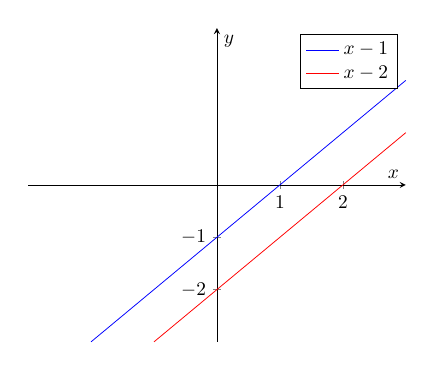
\begin{tikzpicture}[scale=0.7]
            \begin{axis}[
                axis lines = center,
                xlabel = $x$,
                ylabel = $y$,
                xmin=-3, xmax=3,
                ymin=-3, ymax=3,
                clip = false,
                xtick = {1,2},
                ytick = {-2,-1}
            ]
                \addplot[color=blue, samples=2, domain=-2:3]{x-1};
                \addplot[color=red, samples=2, domain=-1:3]{x-2};
    
                \addlegendentry{$x-1$};
                \addlegendentry{$x-2$};
            \end{axis}
        \end{tikzpicture}
    \end{figure}

    \newpage
    
    \item Czy $F$ jest iniekcją lub czy jest surjekcją. \\[10pt]
    Pokażę że $F$ jest iniekcją. \\[5pt] 
    Weźmy $A_1, A_2 \in \Pows (\R)$ takie że $A_1 \neq A_2$. Czyli muszą różnić się co najmniej jednym elementem. Bez straty ogólności założę, że $\Exists_{a_1 \in A_1} \; a_1 \notin A_2$. Więc do $F(A_1)$ należą wszystkie pary liczb rzeczywistych $x, y$ które spełniają $x - y = a_1$, ale do $F(A_2)$ nie należą, więc istotnie $F(A_1) \neq F(A_2)$ co dowodzi że $F$ jest iniekcją. \\[10pt]
    Teraz pokażę że $F$ nie jest surjekcją. \\[5pt]
    Załóżmy przeciwnie że $F$ jest surjekcją i istnieje takie $A \in \Pows (\R)$ że $F(A) = \{\langle 0, 0 \rangle \}$. Z definicji $F$ wiemy że w takim wypadku $0 \in A$, ale wtedy również: 
    $$\{\langle x, y \rangle \in \R^2 \mid x - y = 0\} \subseteq F(A)$$
    Mamy sprzeczność z założeniem, więc nie istnieje takie $A$, więc $F$ nie jest surjekcją. \qed

    \item Udowodnić że $F(\N)$ jest częściowym porządkiem w $\R$ i podać przykład nieskończonego antyłańcucha w tym porządku. \\[10pt]
    Relacja częściowego porządku musi być zwrotna, antysymteryczna i przechodnia.
    \begin{enumerate}[1)]
        \item Zwrotność: \\[5pt]
        Weźmy dowolne $x \in R$. $x - x = 0 \in \N$ więc $\langle x, x \rangle \in F(\N)$.

        \item Antysymetria: \\[5pt]
        Weźmy dowolne $x, y \in \R$ takie że $\langle x, y \rangle \in F(\N)$ i $\langle y, x \rangle \in F(\N)$. Z definicji $F$ to oznacza że $x - y \in \N$ i $y - x \in \N$. Zauważmy że $(x - y) + (y - x) = 0$ Więc są to elementy przeciwne w grupie $(\Z, +, 0)$ Ale jedynym elementem $\Z$ który należy do $\N$ i jego element przeciwny również należy do $\N$ jest $0$, więc $x - y = 0$, a z tego $x = y$.

        \item Przechodniość: \\[5pt]
        Weźmy dowolne $x, y, z \in \R$ takie że $\langle x, y \rangle \in F(\N)$ i $\langle y, z \rangle \in F(\N)$. Z tego wiemy że $x - y \in \N$ i $y - z \in \N$. Teraz dodajmy te dwa elementy do siebie: $(x - y) + (y - z) = x - z$. Korzystając z faktu że zbiór liczb naturalnych jest zamknięty na dodawanie, otrzymujemy $x - z \in \N$. Więc $\langle x, z \rangle \in F(\N)$.
    \end{enumerate}
    Wnioskujemy że istotnie $F(\N)$ jest relacją częściowego porządku. \\[10pt]
    Teraz znaleźć nieskończony antyłańcuch w tym porządku. Rozpatrzmy zbiór $B$:
    $$B = \{a \sqrt{2} \mid a \in \N\}$$
    Niewątpliwie ten zbiór jest nieskończony. Pokażmy że dowolne dwa elementy $B$ nie są porównywalne w porządku $F(\N)$: \\[5pt]
    Weźmy dowolne dwa różne elementy $b_1, b_2 \in B$, takie że $b_1 \neq b_2$ Można je zapisać odpowiednio jako $a_1 \sqrt{2}, a_2 \sqrt{2}$, gdzie $a_1, a_2 \in \N$. Jeśli $b_1 \neq b_2$ to łatwo wywnioskować że $a_1 \neq a_2$. Różnica $b_1 - b_2$ jest równa $(a_1 - a_2) \sqrt{2}$ i jeśli $a_1 \neq a_2$ to ta wartość nigdy nie jest naturalna (to samo dla różnicy $b_2 - b_1$), więc para składająca się z tych dwóch elementów nie jest w zbiorze $F(\N)$ więc nie są porównywalne. \qed

    \item Wyznaczyć przeciwobraz zbioru wszystkich relacji zwrotnych w $\R$ przy funkcji $F$. \\[10pt]
    Oznaczmy zbiór wszystkich relacji zwrotnych jako $\Rel$. Pokażę, że $F^{-1}(\Rel) = \{A \in \Pows(\R) \mid 0 \in A\}$. Dowód poprzez wzajemną inkluzję: \\[5pt]
    $(\subseteq)$ Weźmy dowolne $A \in F^{-1}(\Rel)$. Wiemy że $F(A) = r$ gdzie $r$ jest zwrotne, czyli $\Forall_{x \in \R} \; \langle x, x \rangle \in r$ Ale z definicji $F$ to oznacza że $0 \in A$, więc $A \in \{A \in \Pows(\R) \mid 0 \in A\}$. \\[5pt]
    $(\supseteq)$ Weźmy dowolne $A \in \{A \in \Pows(\R) \mid 0 \in A\}$. Jeśli $0 \in A$ to z definicji $F$ mamy:
    $$\{\langle x, y \rangle \in \R^2 \mid x - y = 0\} \subseteq F(A)$$
    Więc do $F(A)$ należą wszystkie pary postaci $\langle x, x \rangle$ gdzie $x \in \R$. A to oznacza, że jest to relacja zwrotna. Wnioskujemy że $A \in F^{-1}(\Rel)$. \\[5pt]
    Z wzajemnej inkluzji wnioskujemy równość zbiorów. \qed

    \newpage
    
    \item Jakiej mocy jest zbiór $F(\Q)$? \\[10pt]
    Rozważmy funkcję $f \colon \R \times \Q \to F(\Q)$ określoną wzorem:
    $$f(x, q) = \langle x, x - q \rangle$$
    Sprawdźmy czy taka funkcja jest poprawnie zdefiniowana: \\[5pt]
    Weźmy dowolne $x \in \R$ i $q \in \Q$. Mamy $f(x,q) = \langle x, x - q \rangle$, i to musi należeć do $F(\Q)$, więc różnica elementów w parze musi być wymierna: $x - (x - q) = q \in \Q$, więc funkcja jest poprawnie zdefiniowana. \\[5pt]
    Teraz wykażmy jej iniektywność. \\[5pt]
    Weźmy dowolne dwie pary $\langle x_1, q_1 \rangle, \langle x_2, q_2 \rangle \in \R \times \Q$. Jak przyłożymy funkcję $f$ do tych par to otrzymamy odpowiednio $\langle x_1, x_1 - q_1 \rangle$ oraz $\langle x_2, x_2 - q_2 \rangle$. Chcemy aby otrzymane pary nie były równe sobie więc rozpatrzmy dwa przypadki:
    \begin{enumerate}[1)]
        \item $x_1 \neq x_2$: Pierwsze elementy otrzymanych par się różnią, więc wartości funkcji istotnie są różne.

        \item $q_1 \neq q_2$: Jeśli zachodzi również $x_1 \neq x_2$ to lądujemy w przypadku 1) i sprawa jest załatwiona, więc teraz załóżmy $x_1 = x_2$. Pierwsze elementy otrzymanych par są takie same, więc spójrzmy na drugie. Wynoszą odpowiednio $x_1 - q_1$ i $x_2 - q_2$. Łącząc ze sobą dwa założenia $q_1 \neq q_2$ i $x_1 = x_2$ otrzymujemy: $x_1 - q_1 \neq x_2 - q_2$, więc istotnie otrzymane pary są różne.
    \end{enumerate}
    Wnioskujemy że $f$ jest iniekcją. \\[5pt]
    Teraz pokażę jej surjektywność: \\[5pt]
    Weźmy dowolną parę liczb $a, b \in \R$ taką że $\langle a, b \rangle \in F(\Q)$. Z definicji funkcji $F$ musi zachodzić $a - b \in \Q$. Jeśli wezmę $x \in \R$ takie że $x = a$ oraz wezmę $q \in \Q$ takie że $q = a - b$ (istotnie jest to elementem $\Q$ z założenia), to mam $f(x, q) = \langle a, b \rangle$. Więc mamy surjekcję. \\[10pt]
    Więc $f$ jest bijekcją, a co za tym idzie $\R \times \Q \sim F(\Q)$. Z operacji na liczbach kardynalnych mamy:
    $$|\R \times \Q| = |\R| \cdot |\Q| = \cont \cdot \aleph_0 = \cont$$
    Więc $|F(\Q)| = \cont$. \qed
\end{enumerate}
\end{document}
